%! Author = Dean
%! Date = 12/16/2023


\chapter{Neuronske mreže}\label{ch:neuronske-mreze}

Neuronske mreže čine podskup strojnog učenja i predstavljaju temelj algoritama dubokog učenja.
Inspiracija za strukturu i način rada neuronskih mreža crpi se iz ljudskog mozga pokušavajući oponašazi biološke neurone i njihovu međusobnu komunikaciju.


\section{Umjetni neuron}
Prvi model umjetnog neurona je razvijen od strane Warrena McCullocha i Waltera Pittsa, poznat kao McCulloch-Pitts
model umjetnog neurona. Ovaj model oponaša funkcionalnost biološkog neurona, gdje ulazni signali utječu na odluku neurona o tome hoće li
se on aktivirati ili ne
McCulloch-Pitts model umjetnog neurona sastoji se od \textit{n} ulaznih značajki ili signala, označenih s $x_1, x_2, \dots, x_n$, te njihovim pripadajućim težinama $w_1, w_2, \dots, w_n$ koje određuju važnost pojedinih informacija.
\begin{figure}[H]
    \centering
    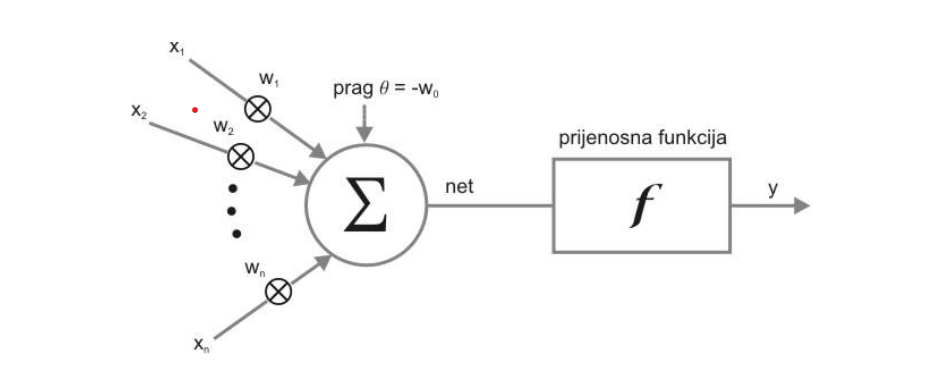
\includegraphics[width=0.8\textwidth]{images/Umjetni_neuron}
    \caption{McCulloch-Pitts model umjetnog neurona}
    \label{fig:slika1}
\end{figure}
Težinska suma neurona \emph{net} se izračunava kao suma ulaznih značajki
\[ net = x_0*w_0 + x_1*w_1 + \dots + x_n*w_n \]
Gdje nam $w_0$ označava takozvana vrijednost praga \emph(bias) koji služi kako bismo odredili kada će neuron biti aktivan ili ne.
Dok nam $x_0$ služi samo radi lakšeg matematičkog zapisa i on je uvijek jedank 1. Znajući sve ovo sad možemo težinsku sumu napisati kao
\[ net = \sum_{i=0}^{\n} w_0*x_0 \]
Drugi način težinske sume koristi vekotorski oblik
\[ net =\vec{w}^T \cdot \vec{x} \]
Na kraju \textit{net} propustimo kroz takozvanu aktivacijsku funckiju \textit{f} koja će nam dati izlaz.

\subsection{Aktivacijska funkcija}
Aktivacijska funkcija je funkcija koja nam daje izlaz neurona na temelju težinske sume.
Glavna uloga aktivacijske funkcije je ta što ona odlučuje hoće li neuron biti aktivan ili ne ili bolje rečeno hoće neuron u toj situaciji biti
važan u ulozi predikcije.
Najjednostavnija moguća aktivacijska funkcija je funkcija identiteta
\[ f(\textit{net}) = net \]
Danas najčešće korištene aktivacijske funkcije us sigmoidalna u ReLU.
Sigmoidalna funkcija je definirana kao:
\[ f(\textit{net}) = \frac{1}{1 + e^-net} \]
\begin{figure}[H]
    \centering
    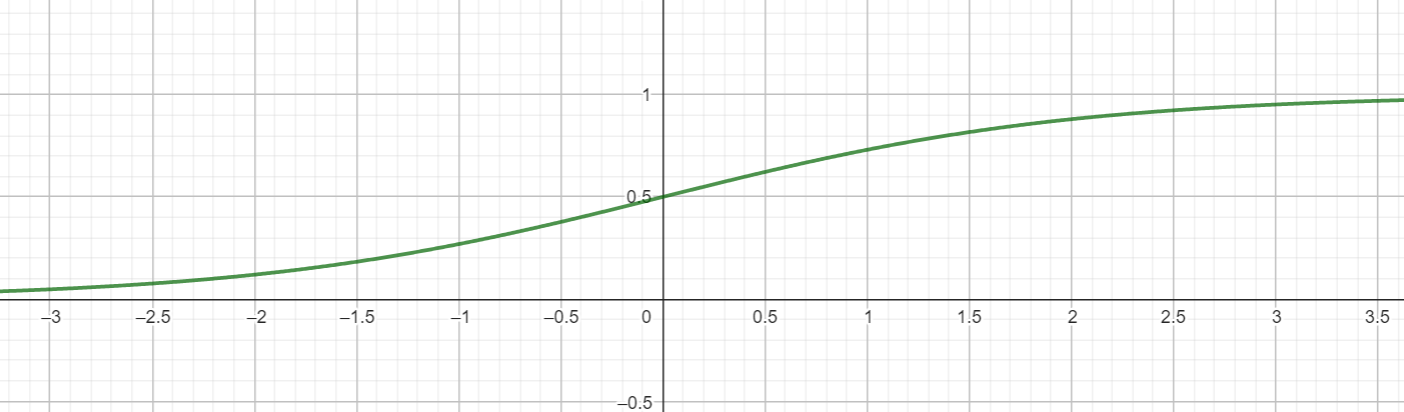
\includegraphics[width=0.8\textwidth]{images/Sigmoid}
    \caption{Sigmoidalna funkcija}
    \label{fig:slika2}
\end{figure}
Kodomena sigmoidalne funkcije je (0, 1) gdje će za jako velike vrijednosti težiti ka 1 a za jako male vrijednosti težiti ka 0.
ReLU aktivacijska funkcija je definirana kao:
\[ f(\textit{net}) = \max(0, \textit{net}) \]
\begin{figure}[H]
    \centering
    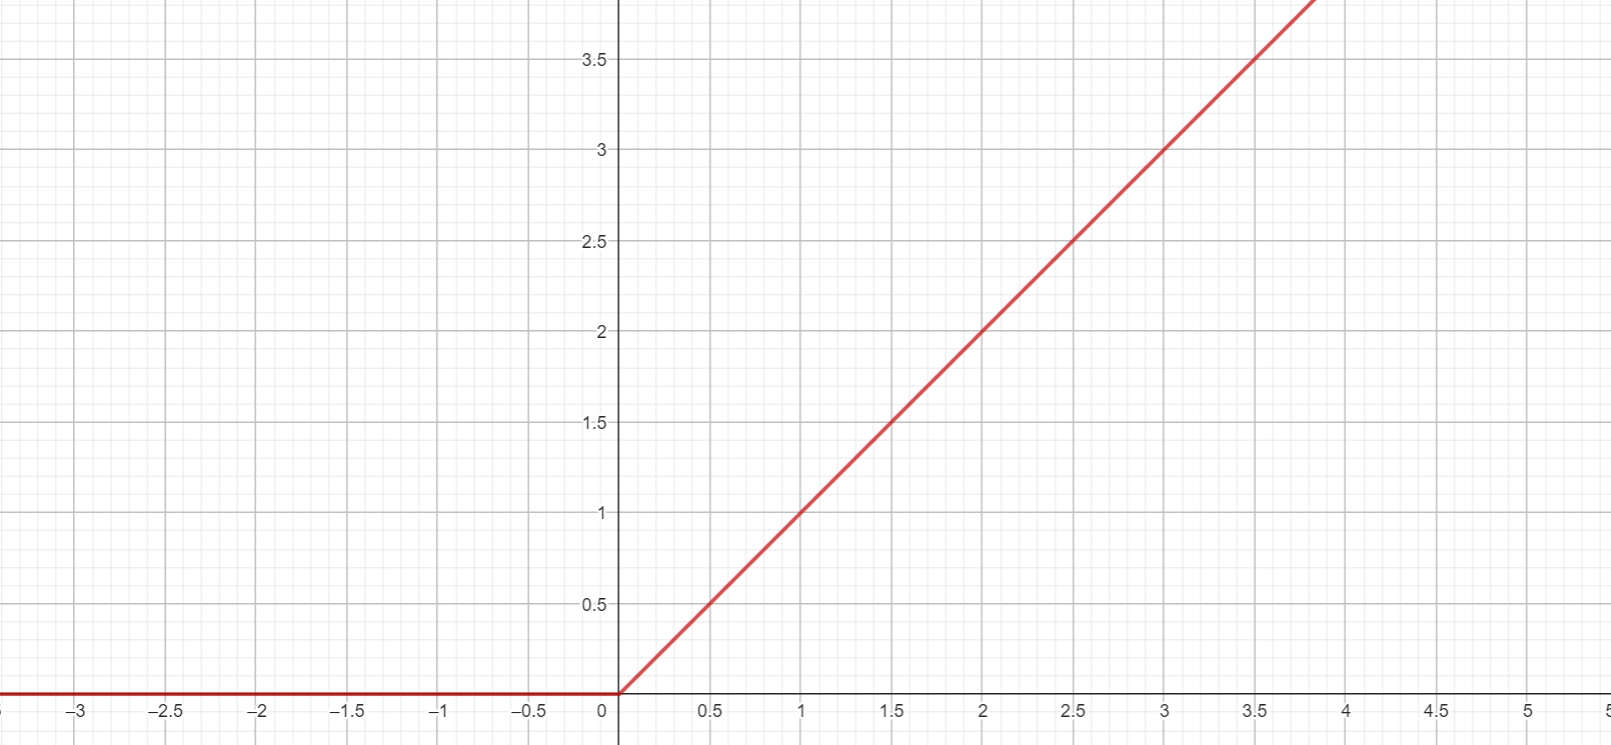
\includegraphics[width=0.8\textwidth]{images/ReLU}
    \caption{ReLU}
    \label{fig:slika3}
\end{figure}

